\section{Implementation Approach}
Clouds are comprehensible indicators for telling the weather. 
They offer many visible features to make an rough prediction of the weather conditions, or weather changes to come.
As described in \sectionref{section:clouds:types}, some cloud types only form under specific conditions.
Also, whenever certain clouds are present, \gls{precipitation} is shortly followed, as it is with altostratus clouds.
\\
Those factors allow a prediction of the weather, but for this project, the process is reversed.
The given data is not an image of clouds, but meteorological measurement data, and the desired outcome is not a prediction, but an image of clouds.

\begin{figure}[H]
    \centering
    \begin{minipage}{0.47\linewidth}
        \begin{tikzpicture}
            \tikzset{edge/.style = {-{Latex[length=3mm]},shorten >= -4pt}}
            \tikzset{shortedge/.style = {shorten <=-4pt,shorten >= -4pt}}
            \tikzset{shortshortedge/.style = {shorten <=-5.5pt,shorten >= -5.3pt}}
            \tikzset{shortshortedge2/.style = {shorten <=-4.5pt,shorten >= -4.5pt}}

            % rainy clouds
            \node (cloud1) at (0.5, 2.0) {};
            \node (cloud2) at (0.8, 2.2) {};
            \node (cloud5) at (1.6, 2.0) {};
            \node (cloud3) at (1.0, 1.9) {};
            \node (cloud4) at (1.3, 2.2) {};
            \node[cloud,fill=gray!30,cloud puffs=9, cloud, minimum width=0.5cm, minimum height=0.2cm, align=center, draw] (cloud) at (cloud1) {};
            \node[cloud,fill=gray!30,cloud puffs=9, cloud, minimum width=0.5cm, minimum height=0.2cm, align=center, draw] (cloud) at (cloud2) {};
            \node[cloud,fill=gray!30,cloud puffs=9, cloud, minimum width=0.5cm, minimum height=0.2cm, align=center, draw] (cloud) at (cloud5) {};
            \node[cloud,fill=gray!30,cloud puffs=12, cloud, minimum width=1.0cm, minimum height=0.7cm, align=center, draw] (cloud) at (cloud3) {};
            \node[cloud,fill=gray!30,cloud puffs=12, cloud, minimum width=0.8cm, minimum height=0.5cm, align=center, draw] (cloud) at (cloud4) {};
            \draw[edge] (2.5, 2) -- (3.5,2);
            \node at (5,2) {rain ahead};

            % clear clouds
            \node (cloud1) at (0.5, 0.0) {};
            \node (cloud2) at (0.9, 0.2) {};
            \node (cloud5) at (1.6, 0.0) {};
            \node[cloud,fill=white,cloud puffs=9, cloud, minimum width=0.5cm, minimum height=0.2cm, align=center, draw] (cloud) at (cloud1) {};
            \node[cloud,fill=white,cloud puffs=9, cloud, minimum width=0.5cm, minimum height=0.2cm, align=center, draw] (cloud) at (cloud2) {};
            \node[cloud,fill=white,cloud puffs=9, cloud, minimum width=0.5cm, minimum height=0.2cm, align=center, draw] (cloud) at (cloud5) {};
            \draw[edge] (2.5, 0) -- (3.5,0);
            \node at (5.7,0) {fair weather ahead};

        \end{tikzpicture}
        \captionof{figure}{Weather information based on visual data.}
        \label{img:tikz:impl:data1}
    \end{minipage}        
    \hfill
    \begin{minipage}{0.47\linewidth}
        \begin{tikzpicture}
            \tikzset{edge/.style = {-{Latex[length=3mm]},shorten >= -4pt}}
            \tikzset{shortedge/.style = {shorten <=-4pt,shorten >= -4pt}}
            \tikzset{shortshortedge/.style = {shorten <=-5.5pt,shorten >= -5.3pt}}
            \tikzset{shortshortedge2/.style = {shorten <=-4.5pt,shorten >= -4.5pt}}

            % rainy clouds
            \node (cloud1) at (4.5, 2.0) {};
            \node (cloud2) at (4.8, 2.2) {};
            \node (cloud5) at (5.6, 2.0) {};
            \node (cloud3) at (5.0, 1.9) {};
            \node (cloud4) at (5.3, 2.2) {};
            \node[cloud,fill=gray!30,cloud puffs=9, cloud, minimum width=0.5cm, minimum height=0.2cm, align=center, draw] (cloud) at (cloud1) {};
            \node[cloud,fill=gray!30,cloud puffs=9, cloud, minimum width=0.5cm, minimum height=0.2cm, align=center, draw] (cloud) at (cloud2) {};
            \node[cloud,fill=gray!30,cloud puffs=9, cloud, minimum width=0.5cm, minimum height=0.2cm, align=center, draw] (cloud) at (cloud5) {};
            \node[cloud,fill=gray!30,cloud puffs=12, cloud, minimum width=1.0cm, minimum height=0.7cm, align=center, draw] (cloud) at (cloud3) {};
            \node[cloud,fill=gray!30,cloud puffs=12, cloud, minimum width=0.8cm, minimum height=0.5cm, align=center, draw] (cloud) at (cloud4) {};
            \draw[edge] (2, 2) -- (3.5,2);
            \node at (0,2) {rain ahead};

            % clear clouds
            \node (cloud1) at (4.5, 0.0) {};
            \node (cloud2) at (4.9, 0.2) {};
            \node (cloud5) at (5.6, 0.0) {};
            \node[cloud,fill=white,cloud puffs=9, cloud, minimum width=0.5cm, minimum height=0.2cm, align=center, draw] (cloud) at (cloud1) {};
            \node[cloud,fill=white,cloud puffs=9, cloud, minimum width=0.5cm, minimum height=0.2cm, align=center, draw] (cloud) at (cloud2) {};
            \node[cloud,fill=white,cloud puffs=9, cloud, minimum width=0.5cm, minimum height=0.2cm, align=center, draw] (cloud) at (cloud5) {};
            \draw[edge] (2.5, 0) -- (3.5,0);
            \node at (0.7,0) {fair weather ahead};
            
        \end{tikzpicture}
        \captionof{figure}{Visual construction based on weather information.}
        \label{img:tikz:impl:data2}       
    \end{minipage}
\end{figure}

\noindent
For any given day to render, an implementation would require data from that day but also from the near future of that day.
So, in order to render a cloud image for day $x$, a potential algorithm could look like this.
Note that the listing below describes only an idea and is by no means final or compulsory.

\begin{lstlisting}[language=HLSL, caption=Pseudo-code of cloud render algorithm., label=lst:pseudo:algorithm]
// weather data including 7-day forecast
WeatherData data;

function renderClouds(Day x) {
    if (x > TODAY + 7) throw;

    d1 = data.getDataFor(x);
    d2 = data.getDataFor(x + 1);
    d3 = data.getDataFor(x + 2);
    // and so on...

    // sophisticated checks about current and future conditions:
    if (d1.fairWeather && d2.fairWeather)
        return renderer.clearSky();
    if (d1.fairWeather && d2.isRaining)
        return renderer.cloudsOnclearDayBeforeRain();
    if (d1.isRaining)
        return renderer.cloudsOnRainyDay();
    if (d2.isRaining) 
        return renderer.cloudsBeforeRainyDay();
    if (d3.isRaining) 
        return renderer.clouds2DaysBeforeRainyDay();
    // and so on...
    
}
\end{lstlisting}

\clearpage

\subsection{Look-Ahead Issue}
The approach as described above relies on having data from a couple of days ahead of time. Assumed that number of days is $t$, then the weather data for day $x$ could only be rendered $t$ days after $x$.
That would mean, for such an approach to work, the weather of today can not be rendered before $t$ days later.
\\
In this case however, the weather measurement data retrieved from \emph{meteoblue} also contains a seven-day weather forecast. 
Given that $t$ is less than or equal to seven and an implementation still produces accurate cloud imagery, it would no longer be an issue.

\subsection{Layers of Cloud Shaders}
As identified in \sectionref{section:clouds:types}, most of the clouds in the troposhpere only appear at certain \gls{altitude}s.
The high-level clouds are all of type \emph{cirrus}.
The mid-level types are altostratus and altocumulus, while the low-level types are stratus, stratocumulus and stratus.
\\
This leads to the conclusion that some of the cloud types could be consolidated into a combined layer and rendered by the same shader.
Exception to that are only the two larger types that span over multiple height levels: nimbostratus and cumulonimbus. For those, a more unique solution has to be found.

\begin{figure}[H]
    \centering
    \begin{tikzpicture}[scale=1]
        \tikzset{edge/.style = {-{Latex[length=3mm]},shorten >= -4pt}}
        \tikzset{shortedge/.style = {shorten <=-4pt,shorten >= -4pt}}
        \tikzset{icon/.style = {font=\Large}}

        % icons
        \node[red,icon] (cam) at (0.1, 5.2) {\faVideoCamera};
        \node[red,yshift=-0.5cm,xshift=-0.3cm] at (cam) {camera};
        \draw (0.5,5.45) -- (2,7);
        \draw (0.5,4.95) -- (2,3.5);

        % cloud layer boxes
        \draw (3,7) rectangle (8,6.2);
        \draw (3,6) rectangle (8,5.2);
        \draw (3,5) rectangle (8,4.2);
        \draw (3,4) rectangle (11,2.2);
        \draw (8.2,7) rectangle (11,4.2);
        \node at (5.5,6.6) {high-level clouds};
        \node at (5.5,5.6) {mid-level clouds};
        \node at (5.5,4.6) {low-level clouds};
        \node at (6.8,3.1) {ground level fog};
        \node[text width=2cm] at (10,5.6) {cumulo-nimbus};

        % houses
        \node[black!40] at (4.9, 1.15) {\faHome};
        \node[black!40] at (5.2, 1.20) {\faHome};
        \node[black!40] at (5.4, 1.24) {\faHome};
        \node[black!40,icon] at (5.7, 1.25) {\faHome};
        \node[black!40] at (6.0, 1.15) {\faHome};
        \node[black!40] at (6.35, 1.22) {\faHome};
        \node[black!40] at (6.8, 1.4) {\faUniversity};
        \node[black!40] at (7.1, 1.32) {\faHome};
        \node[black!40] at (7.5, 1.25) {\faHome};
        \node[black!40,icon] at (7.8, 1.23) {\faHome};
        \node[black!40] at (8.1, 1.16) {\faHome};
        \node[black!60] at (6.4,0.7) {city of Bern};
        
        % ground
        \node[green!50!black,rotate=-58,anchor=west] at (1.2,3.1) {ground};
        \draw[green!50!black,thick] (0,4.2) -- (0.2,4.2) -- (0.4,4.1) -- (0.5,4) -- (1,3) -- (2,1.5) -- (3,1.1) -- (5,1) -- (5.1,1.05) -- (5.4,1.1) -- (6,1) -- (6.5,1.1) -- (6.6,1.2) -- (7,1.2) -- (8,1) -- (10,1.1) -- (12,1);

        % height of troposphere
        \draw (13.0,1) -- (13.0,7);
        \draw (13.1,1) -- (12.9,1);
        \draw (13.1,7) -- (12.9,7);
        \node[rotate=90,anchor=west] at (12.7,2.5) {troposphere height};

    \end{tikzpicture}
    \captionof{figure}{Layers of cloud shaders.}
    \label{img:tikz:shadersetup}       
\end{figure}

\pagebreak

\subsubsection{High-Level Clouds}
The uppermost layer would contain cirrus, cirrostratus and cirrocumulus clouds.
All of these form under similar weather conditions and closely resemble each other in appearance and formation.
\\
A potential \gls{shader} for that layer could be programmed to render a base variant of all three cirrus clouds, which would then be parametrized into each individual type of cirrus cloud, whichever is currently visible.

\begin{figure}[H]
    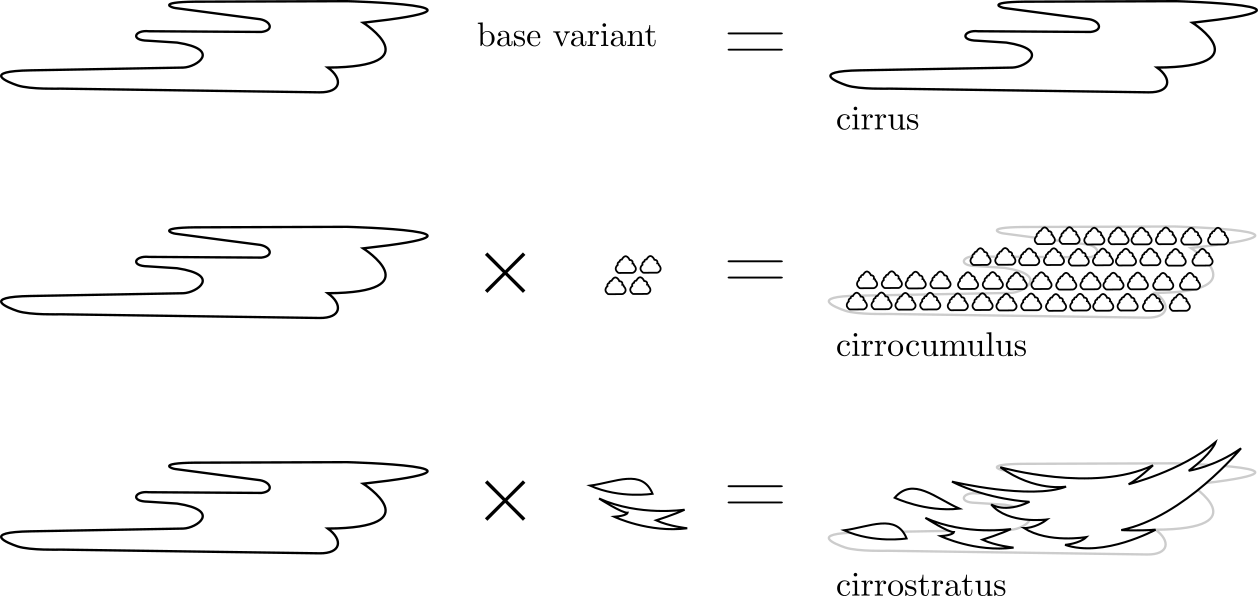
\includegraphics[width=\linewidth]{cloudlayers/cirruslayer.png}
    \caption{Breakdown of the highest shader layer.}
    \label{img:cloudlayer:cirrus}
\end{figure}

\subsubsection{Mid-Level Clouds}
The middle layer consists of altostratus and altocumulus clouds, the latter mainly occuring due to dissipation of the former one.
Since they have many shared characteristics, apart from the density, they are predestined to be processed together.
\\
Given a \gls{shader} is flexible enough to render altostratus clouds, then it is most likely also able to render altocumulus, with only few adjustements necessary.

\begin{figure}[H]
    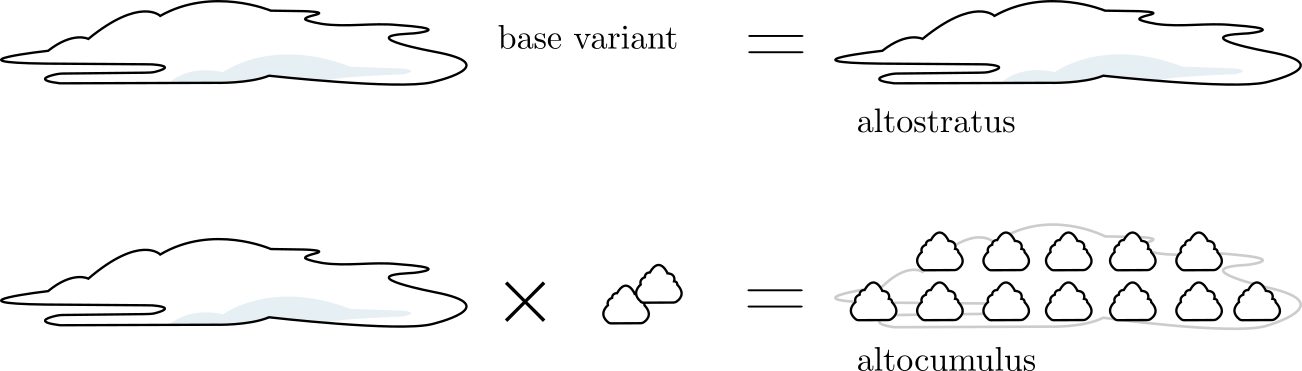
\includegraphics[width=\linewidth]{cloudlayers/altolayer.png}
    \caption{Breakdown of the middle shader layer.}
    \label{img:cloudlayer:alto}
\end{figure}

\pagebreak

\subsubsection{Low-Level Clouds}
The lower layer may prove to be more complex than the others, as the stratus and cumulus clouds do essentially not look alike.
However, cumulus clouds could be described as less denser, smaller and separated instances of stratocumulus clouds.
\\
If a \gls{shader} would be able to render stratocumulus clouds and allow to control the density or the spreading of such, then cumulus clouds could be rendered in the same manner.

\begin{figure}[H]
    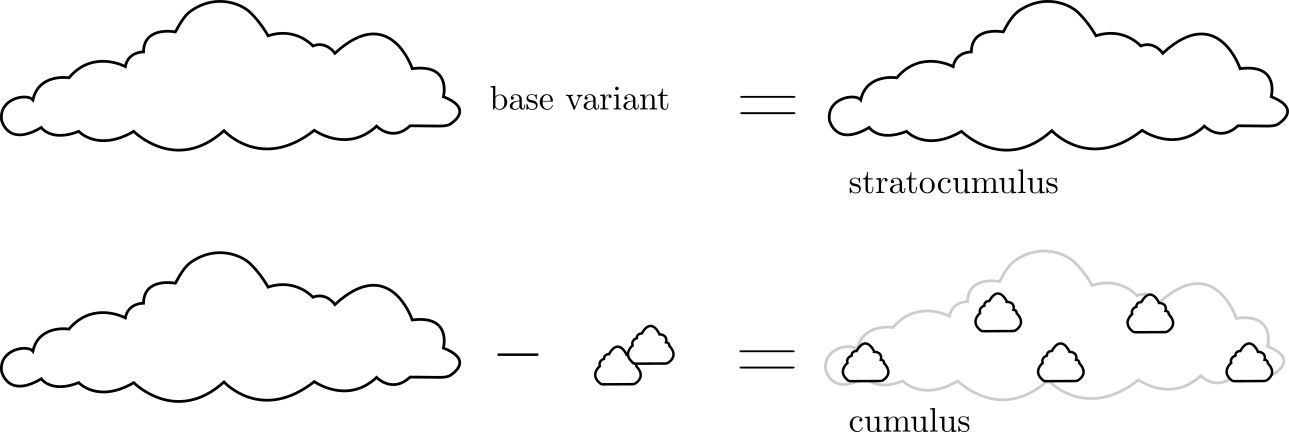
\includegraphics[width=\linewidth]{cloudlayers/stratolayer.png}
    \caption{Breakdown of the lowest shader layer.}
    \label{img:cloudlayer:alto}
\end{figure}


\subsubsection{Ground Level Fog}
The lowest layer consists of fog. It is conceivable that stratus clouds will also be placed in that layer.
Both type of clouds are to some extent combinable, as they primarily vary in density.
\\
Therefore, a \gls{shader} would need to have control over the outcome's density and lightness for it to be able to render both stratus clouds and ground fog.

\begin{figure}[H]
    
\includegraphics[width=\linewidth]{cloudlayers/foglayer.png}
    \caption{Breakdown of the fog shader layer.}
    \label{img:cloudlayer:fog}
\end{figure}

\pagebreak

\subsubsection{Cumulonimbus Layer}
With all the previous layers implemented, only the two large cloud types are left, one of them is the cumulonimbus.
\\
Assuming the observer is walking directly underneath a cumulonimbus cloud, the cloud itself and its defining visual features are not really reckognizable.
It could easily be mistaken for other clouds that produce \gls{precipitation}.

\begin{figure}[H]
    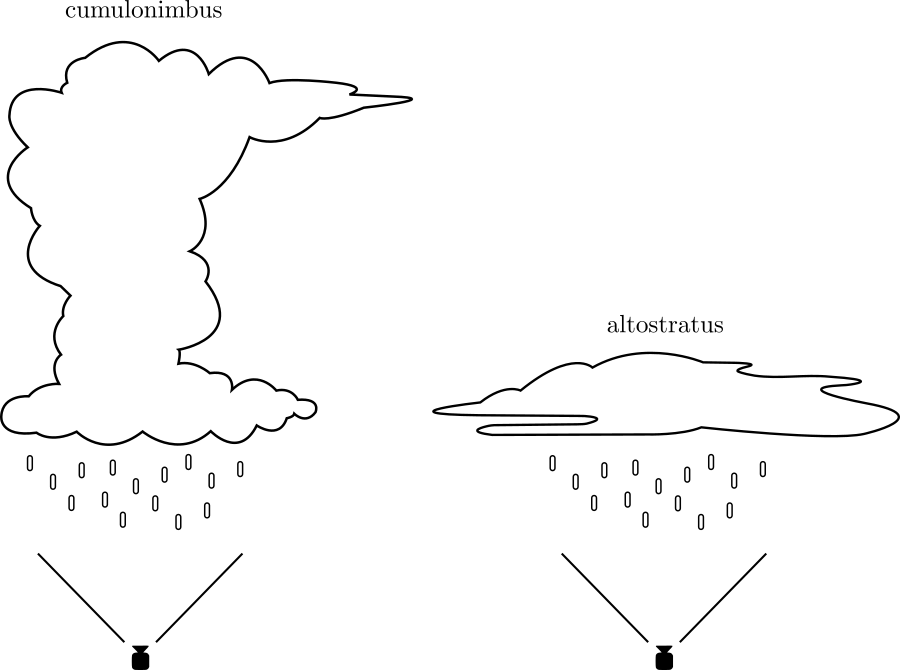
\includegraphics[width=\linewidth]{cloudlayers/cumulonimbus.png}
    \caption{Perspective similarities under clouds with \gls{precipitation}.}
    \label{img:cloudlayer:cumulonimbus}
\end{figure}

\noindent
Under that assumption, it is considered that the cumulonimbus cloud will only ever be seen from a distance.
This is why these clouds will most likely be rendered in their own layer, farther away from the main camera, but spanning over all other height levels.

\pagebreak

\subsubsection{Nimbostratus Layer}
A similar issue as with the cumulonimbus clouds is present for the nimbostratus clouds.
Due to them being thick, dark layers of cloud lacking features and contours, they are more difficult to render.
\\
It is, however, imaginable to omit the type nimbostratus altogether and substitute it by combining and tuning the already existing layers.
For example, the nimbostratus cloud might be imitated by darkening the color of altostratus clouds as well making them thicker. 
With additional stratus clouds and increased fog density, a layman could hopefully no longer tell the difference.

\begin{figure}[H]
    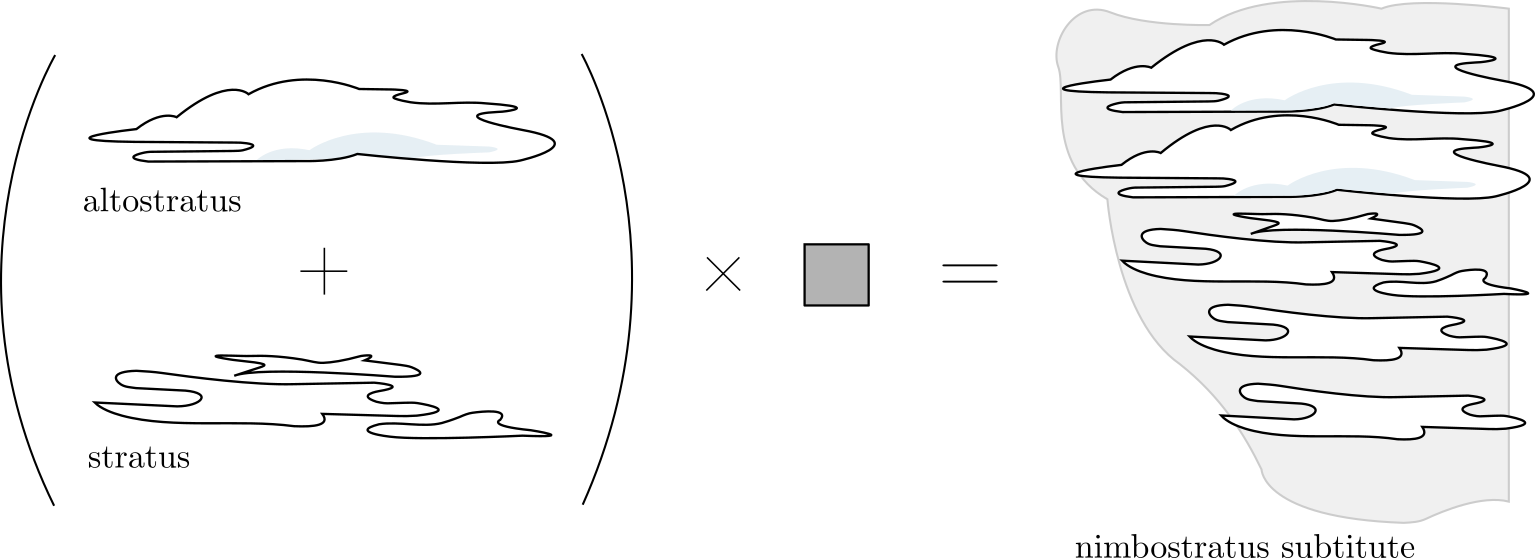
\includegraphics[width=\linewidth]{cloudlayers/nimbostratus.png}
    \caption{Breakdown of the nimbostratus substitute.}
    \label{img:cloudlayer:nimbostratus}
\end{figure}